\chapter{Calibrazione}\label{ch:calibrazione}

% I dati a disposizione
\section{I dati a disposizione}\label{sec:dati}
\ldots

\subsection{Dataset NO2}\label{ssec:dataset-no2}
\ldots

\subsection{Dataset PM2.5 e PM10}\label{ssec:dataset-pm}
\ldots

\subsection{Preprocessamento}\label{ssec:preprocessamento}
\ldots

% Regressione
\section{Regressione}\label{sec:regressione}
Nella statistica applicata come nelle scienze sperimentali si osserva (o si ipotizza) l’esistenza di relazioni fra due o più grandezze.

Sorge allora il problema di determinare una funzione che, in base ai dati ricavati mediante esperimenti o rilevazioni statistiche, rappresenti questi relazioni permettendo, in questo modo, di analizzare meglio i fenomeni osservati.

Limitando lo studio a problemi che stabiliscono relazioni fra due sole variabili, si tratta, partendo dalle coppie $(x_i, y_i)$ di dati corrispondenti rilevati, di determinare una funzione $y=f(x)$ che rappresenti il fenomeno.

Per trovare una funzione che rappresenti il fenomeno si può procedere in due modi:

\begin{itemize}
  \item determinare una funzione che assuma esattamente i valori $(x_i, y_i)$ rilevati; questo procedimento viene detto interpolazione per punti noti;
  \item determinare una funzione che si accosti il più possibile ai punti $(x_i, y_i)$; questo procedimento viene detto interpolazione fra punti noti.
\end{itemize}

La ricerca di una funzione, generalmente espressa da un polinomio, che passi esattamente per i punti $(x_i, y_i)$ è piuttosto laboriosa; nelle applicazioni statistiche si preferisce determinare una funzione il cui grafico si avvicini ai punti rilevati.

Osservando l’andamento del fenomeno si sceglie il tipo di funzione interpolatrice: lineare, quadratica, esponenziale, ecc. e quindi si procede alla determinazione dei parametri, ossia delle costanti che compaiono nella funzione scelta in modo che sia soddisfatta una condizione di accostamento prefissata.

Per conseguire questo scopo il metodo più utilizzato è il metodo dei \textbf{minimi quadrati} che costituisce un’applicazione della ricerca del minimo di una funzione di più variabili mediante gli strumenti dell’analisi infinitesimale.

Si considerino due variabili $X$ e $Y$ sulle quali si sono effettuate $n$ rilevazioni: $$\left(x_{1}, y_{1}\right),\left(x_{2}, y_{2}\right), \ldots,\left(x_{i}, y_{i}\right), \ldots,\left(x_{n}, y_{n}\right)$$

Sia $y=f(x; a, b, c, ..., k)$ la funzione interpolatrice scelta. Siano inoltre $\hat{y}_{i}$ valori teorici sulla curva corrispondenti ai valori $x_i$ rilevati.

La condizione di accostamento data dal metodo dei minimi quadrati è quella di determinare i valori dei parametri in modo che sia minima la somma dei quadrati delle differenze fra i valori osservati $y_i$ e i valori teorici $y_i$ (figura \ref{fig:minimi_quadrati}), ovvero:

$$\varphi(a, b, c, \ldots, k)=\sum_{i=1}^{n}\left[y_{i}-f\left(x_{i} ; a, b, c, \ldots, k\right)\right]^{2}$$

dove i valori $x_i$ e $y_i$ sono noti, mentre sono incogniti i parametri $a , b , c , … , k$ della funzione. \cite{excel_per_statistica_belluco}

\begin{figure}[H]
\centering
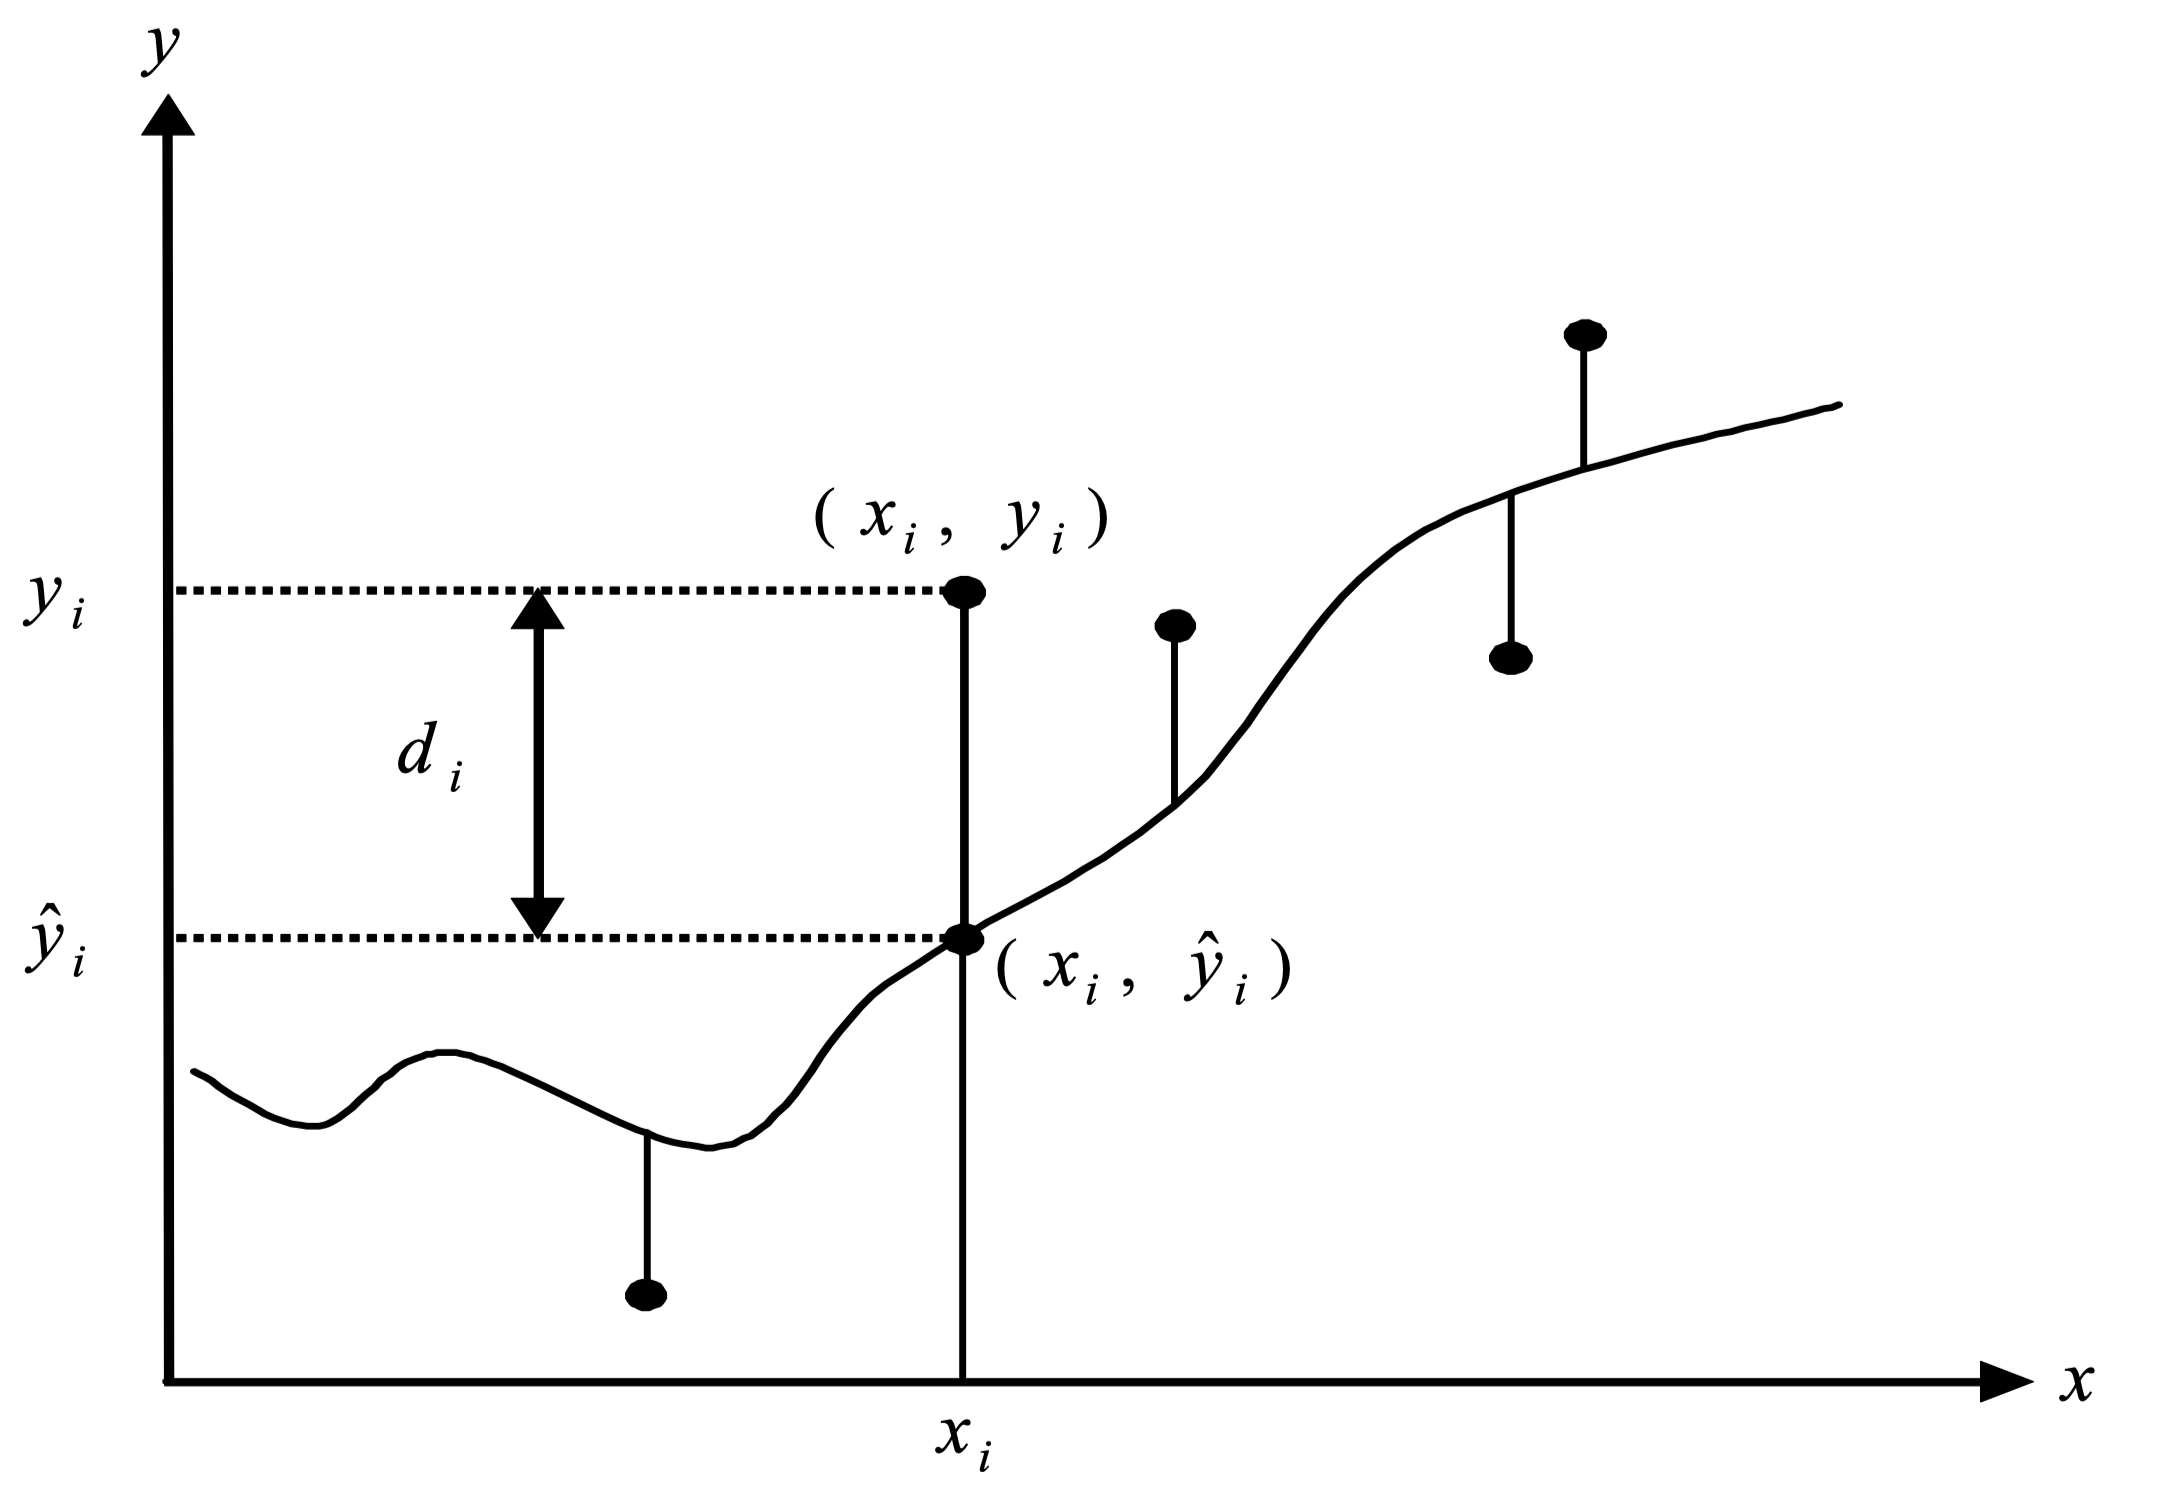
\includegraphics[width=0.75\textwidth,height=\textheight,keepaspectratio]{img/minimi_quadrati.png}
\caption{Condizione dei \textit{minimi quadrati} \cite{excel_per_statistica_belluco}}
\label{fig:minimi_quadrati}
\end{figure}

\subsection{Correlazione e analisi}\label{ssec:regressione-analisi}

Quando la dipendenza tra le due variabili è lineare, si parla di correlazione lineare, che può essere valutata mediante il coefficiente di correlazione lineare ($r$):

$$r=\frac{\sum_{i=1}^{n}\left(x_{i}-\bar{x}\right)\left(y_{i}-\bar{y}\right)}{\sqrt{\sum_{i=1}^{n}\left(x_{i}-\bar{x}\right)^{2}} \sqrt{\sum_{i=1}^{n}\left(y_{i}-\bar{y}\right)^{2}}}$$\smallskip

dove il termine al numeratore rappresenta la \textit{covarianza} di $X$ ed $Y$ cioè la variabilità congiunta delle coppie ($x_i$, $y_i$) di valori corrispondenti rispetto al proprio valor medio; mentre il denominatore rappresenta il prodotto delle deviazioni standard di $X$ ed $Y$.

Il coefficiente di correlazione lineare gode di importanti proprietà:

\begin{itemize}
  \item $-1 \le r \le 1$;
  \item si ha $r=1$ quando tutti i dati sono allineati lungo una retta crescente (figura \ref{fig:positive_correlation});
    \begin{figure}[H]
\centering
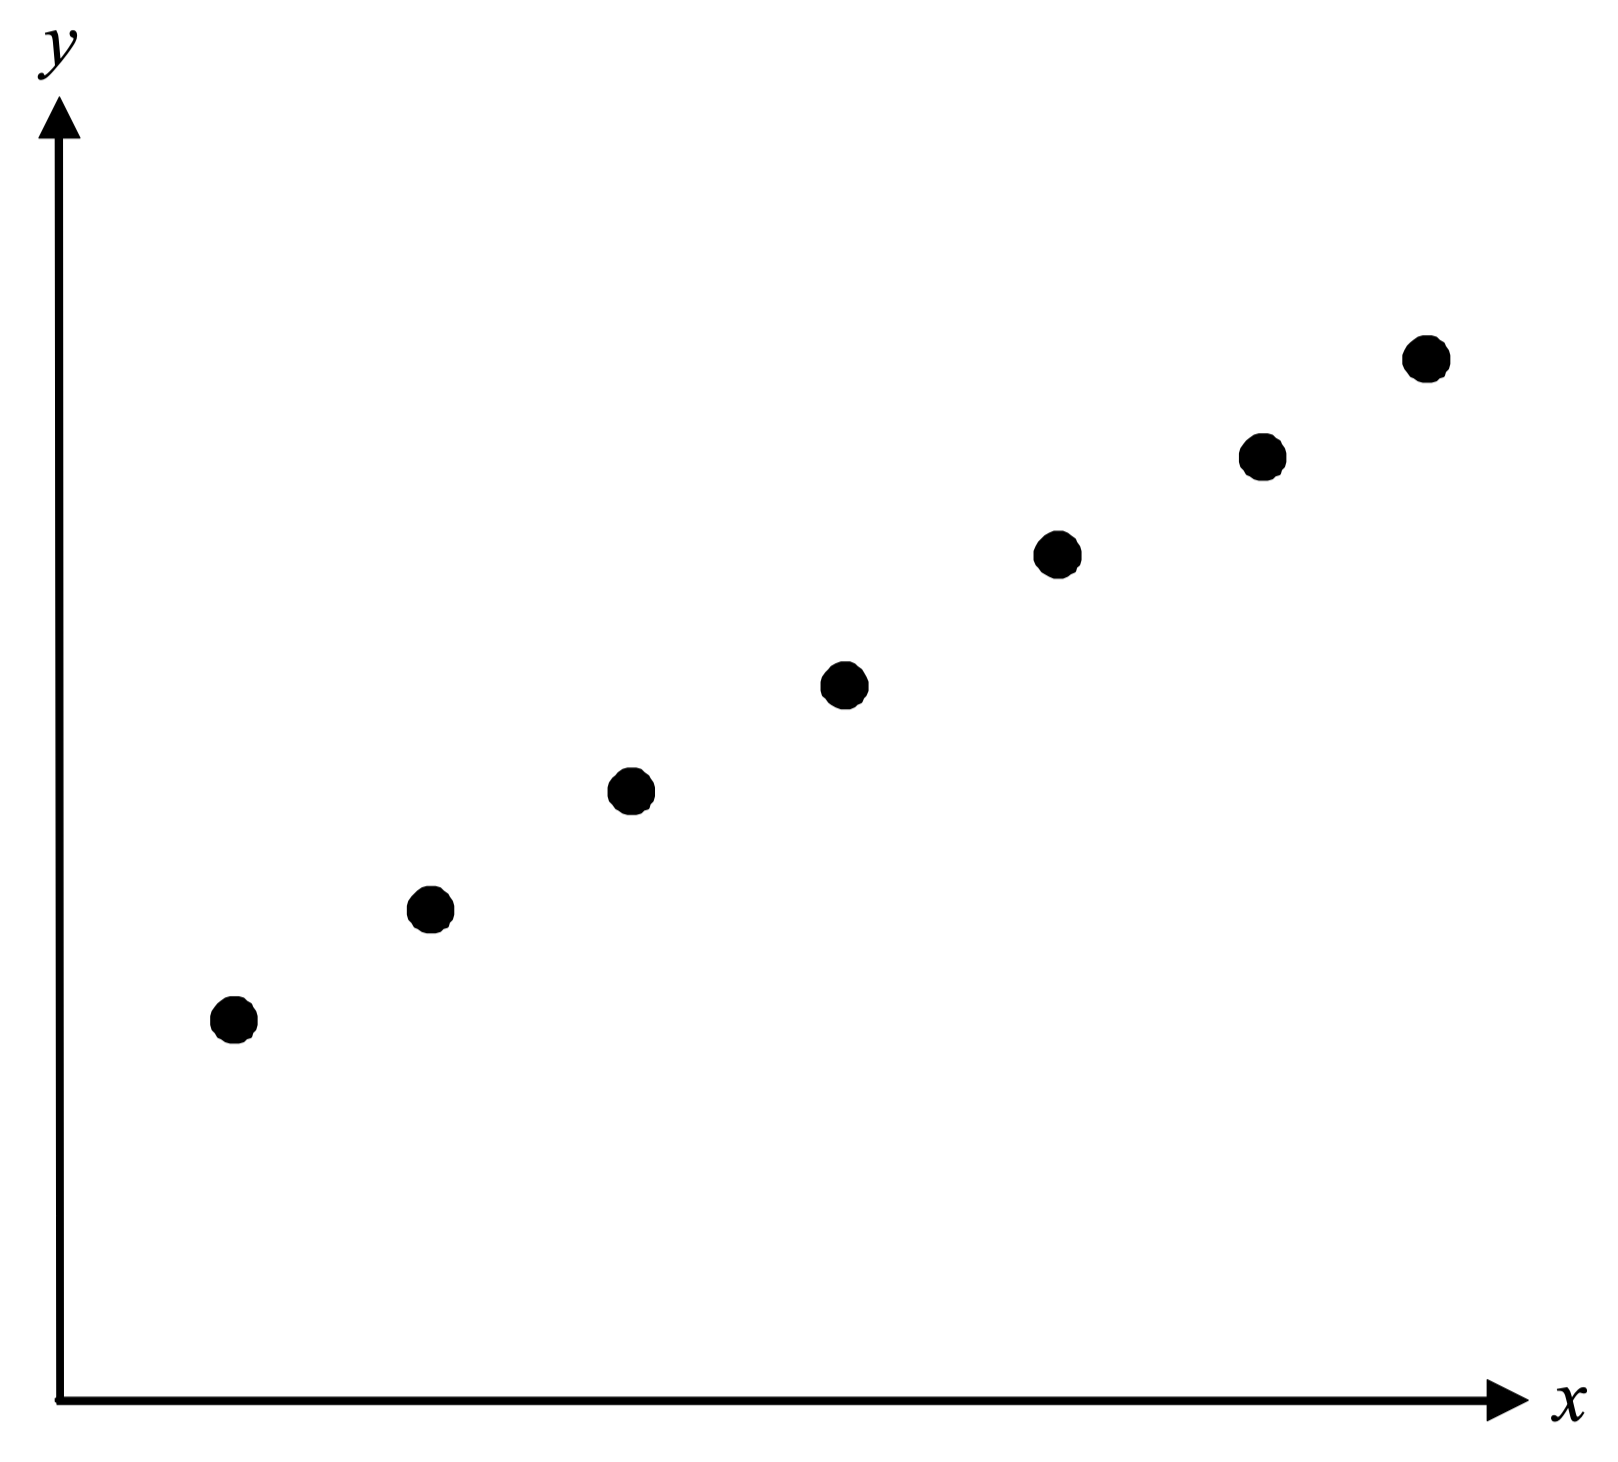
\includegraphics[width=0.55\textwidth,height=\textheight,keepaspectratio]{img/positive_correlation.png}
\caption{Correlazione lineare positiva}
\label{fig:positive_correlation}
\end{figure}

  \item si ha $r=-1$ quando tutti i dati sono allineati lungo una retta decrescente  (figura \ref{fig:negative_correlation});
      \begin{figure}[H]
\centering
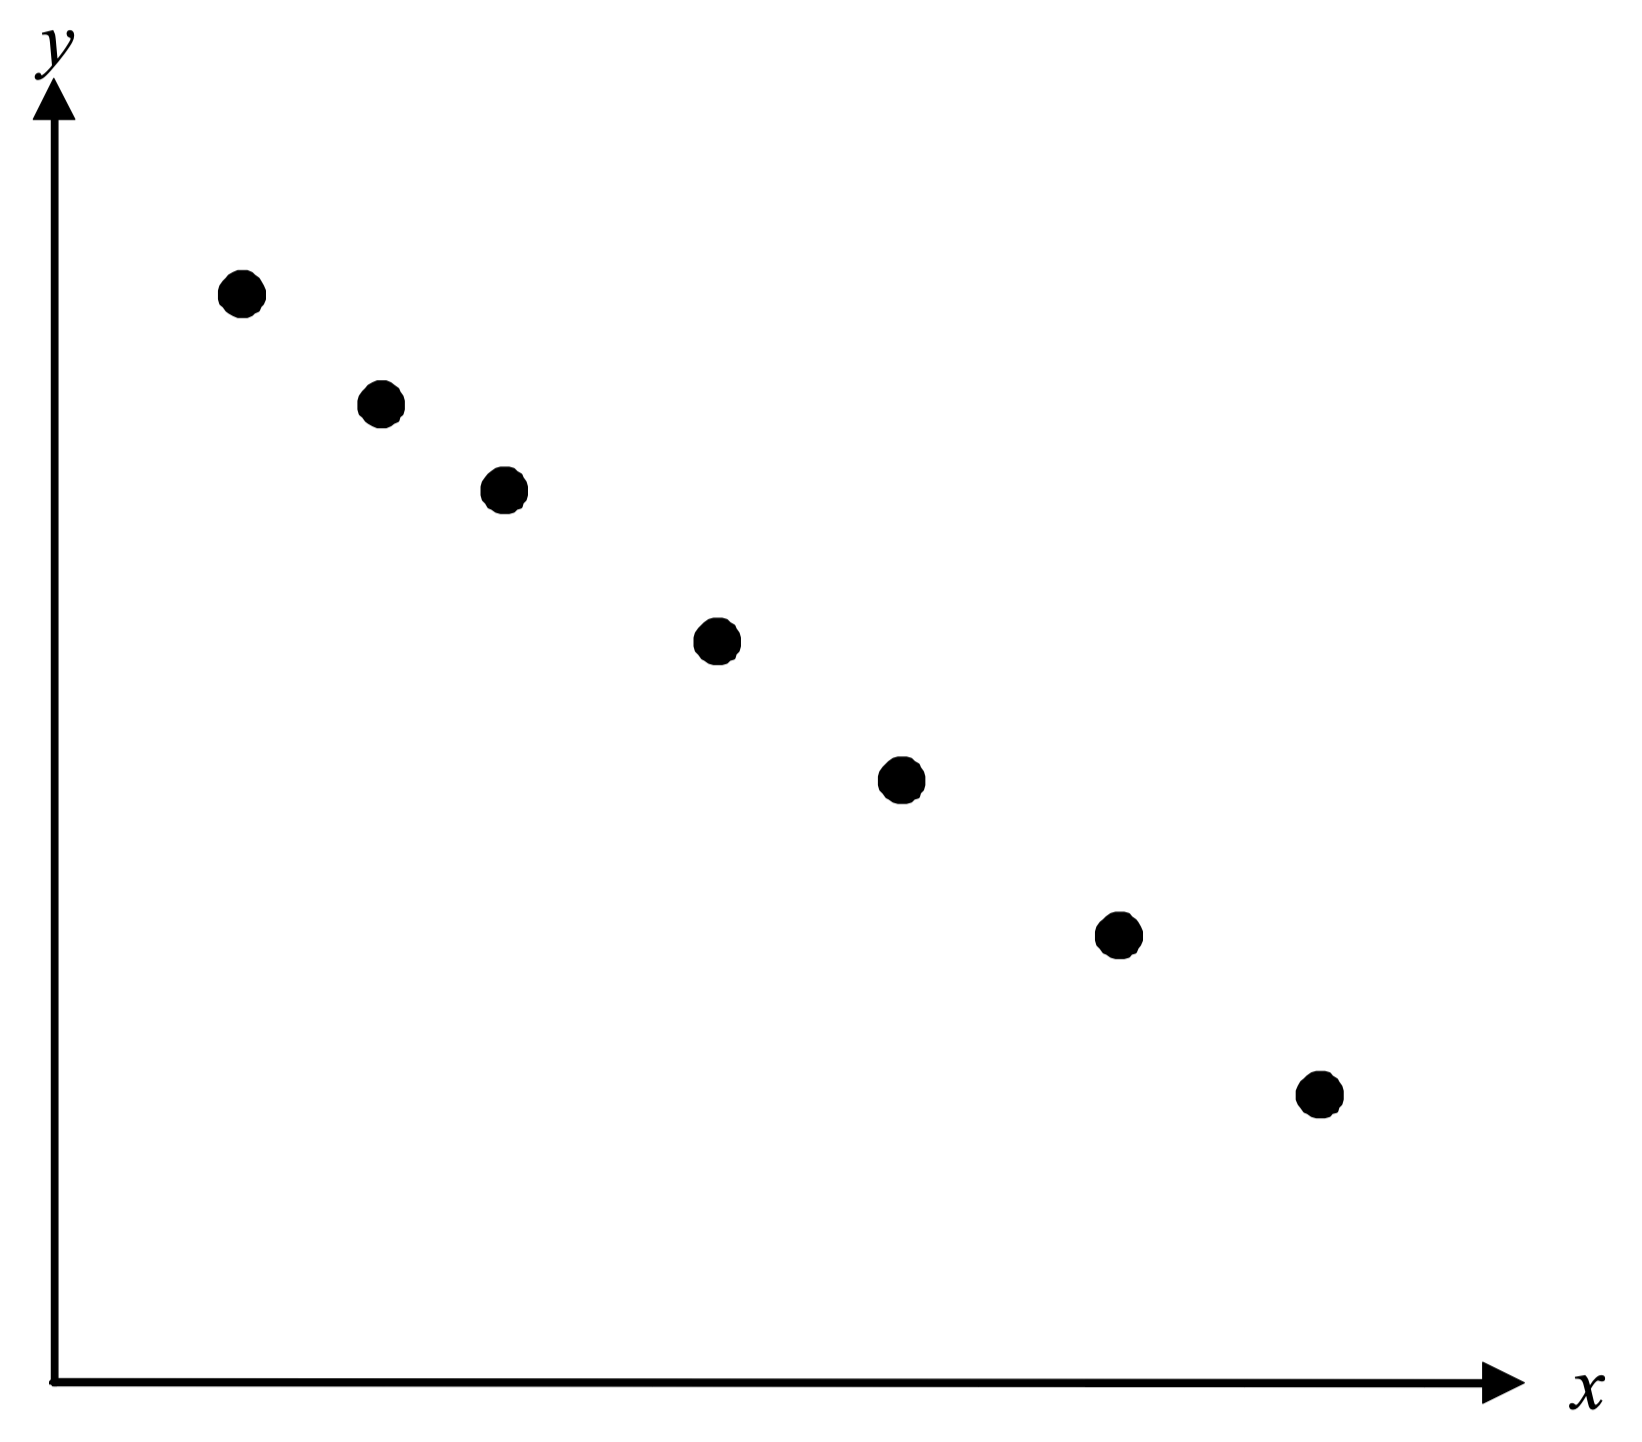
\includegraphics[width=0.55\textwidth,height=\textheight,keepaspectratio]{img/negative_correlation.png}
\caption{Correlazione lineare negativa}
\label{fig:negative_correlation}
\end{figure}
  \item si ha $r=0$ quando non esiste una relazione lineare tra i dati  (figura \ref{fig:no_correlation}).
  \begin{figure}[H]
\centering
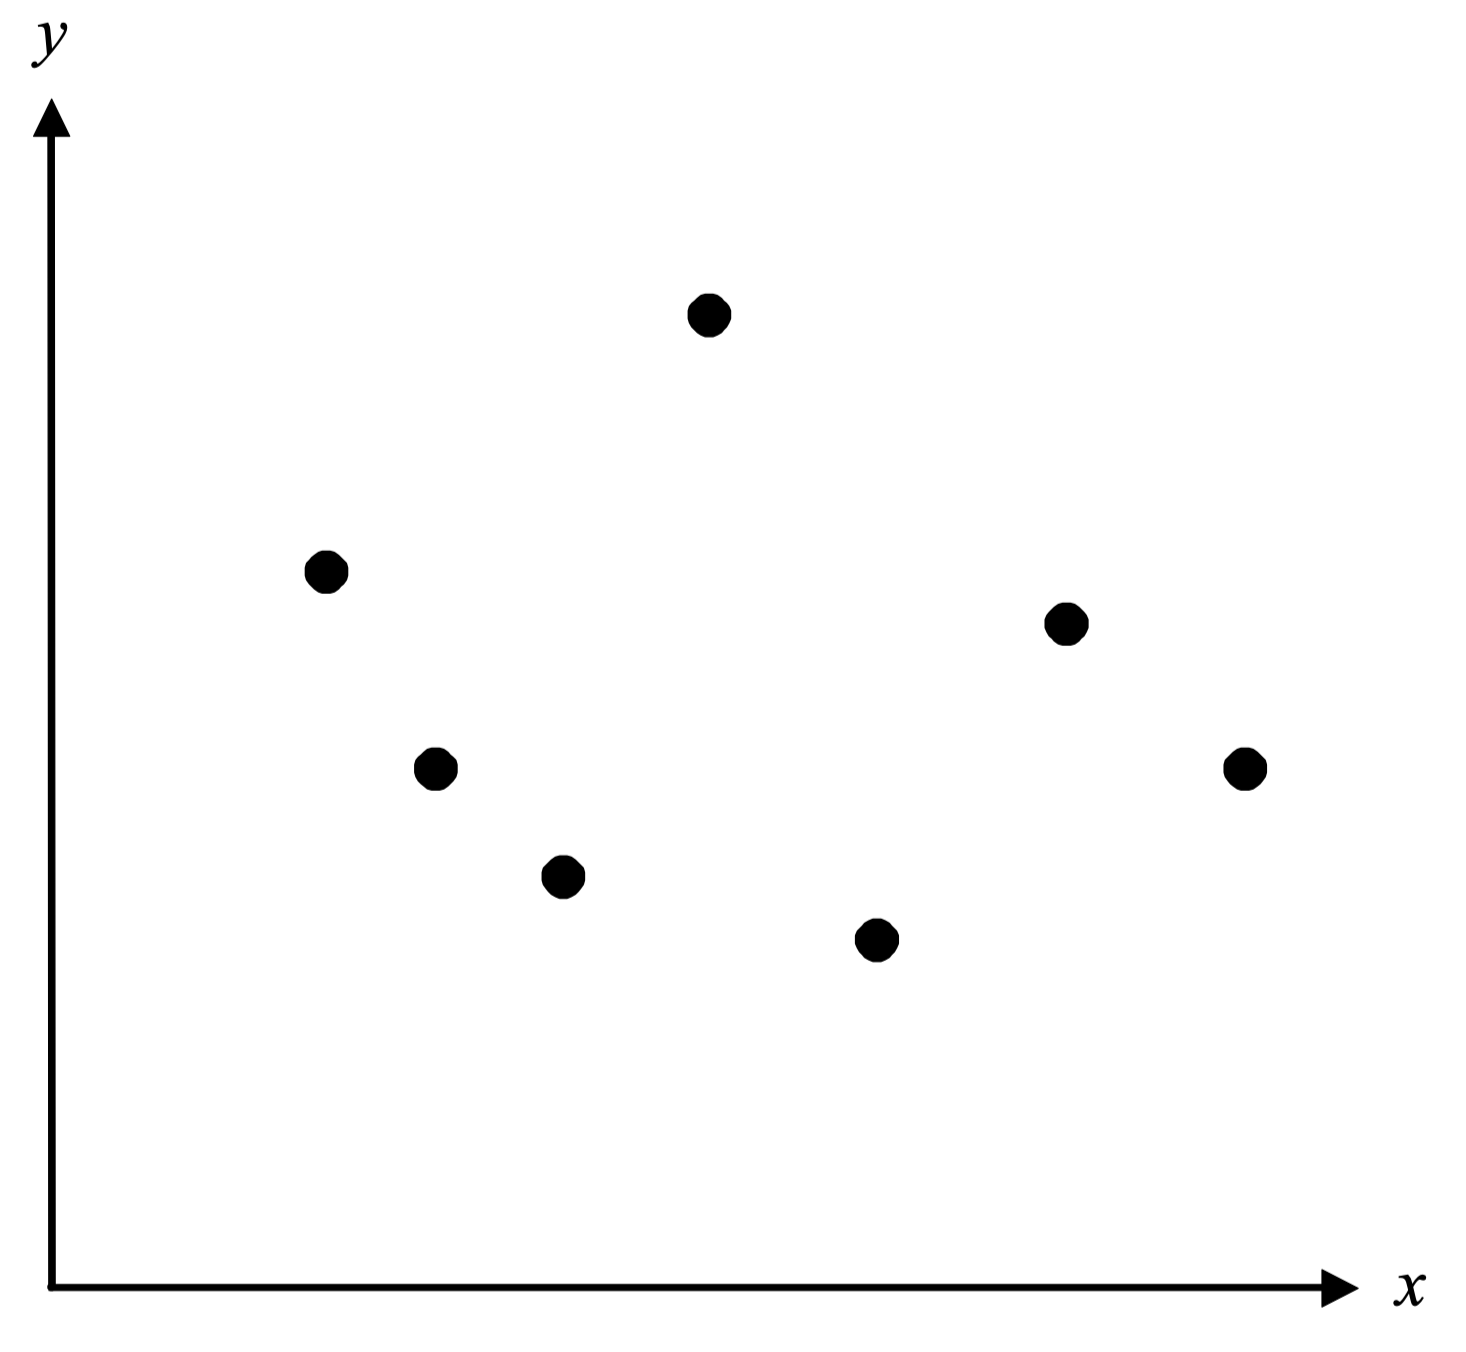
\includegraphics[width=0.55\textwidth,height=\textheight,keepaspectratio]{img/no_correlation.png}
\caption{Nessuna correlazione}
\label{fig:no_correlation}
\end{figure}
\end{itemize}

Sapendo che la varianza ($\sigma_{y}^{2}$) della variabile $Y$ si può scomporre in una parte ($\sigma_{\hat{y}}^{2}$), detta varianza spiegata, in quanto la variabilità della $Y$ è dovuta alla dipendenza di $Y$ dalla variabile $X$, e in una parte ($\sigma_{e}^{2}$), detta varianza non spiegata, in quanto la variabilità della $Y$ non dipende dalla variabile $X$, ma da altri fattori; si può introdurre un secondo indicatore, dato dal rapporto tra la varianza spiegata e la varianza totale, chiamato coefficiente di determinazione:

$$r^{2}=\frac{\sigma_{\hat{y}}^{2}}{\sigma_{y}^{2}}$$\smallskip

che indica quale frazione di varianza totale è dovuta alla dipendenza fra le variabili $Y$ e $X$, ossia quale frazione della variazione della variabile Y è spiegata dalle variazioni della variabile $X$.

Sapendo che:

$$\sigma_{y}^{2}=\sigma_{\hat{y}}^{2}+\sigma_{e}^{2}$$

allora:

$$r^{2}=\frac{\sigma_{\hat{y}}^{2}}{\sigma_{\hat{y}}^{2}+\sigma_{e}^{2}}$$\smallskip

è evidente, quindi, che se la variabilità non spiegata è trascurabile, $\sigma_{e}^{2}$ tende ad annullarsi ed $r^{2}$ avrà un valore prossimo ad 1, mentre diverrà via via minore di 1 al diminuire dell’accordo tra la funzione calcolata e le osservazioni sperimentali.

Minore è la somma residua rispetto alla somma totale dei quadrati, maggiore sarà il valore del coefficiente di determinazione, $r^2$, il quale è un indicatore del livello di precisione con cui l'equazione ottenuta dall'analisi di regressione spiega la relazione tra le variabili.

%La regressione è una tecnica statistica che serve a stimare la relazione esistente tra due o più variabili. In particolare, la regressione permette di individuare il coefficiente di correlazione tra due variabili e di determinare se questa relazione è casuale o no.
%
%Tra le applicazioni principali della regressione ci sono:
%
%- Stima della relazione tra due variabili
%
%- Analisi della relazione tra variabili
%
%- Valutazione dell'influenza di una variabile sulle altre
%
%- Predicting

\subsection{Modelli di regressione}\label{ssec:regressione-modelli}
\ldots

\subsubsection{Regressione lineare}\label{sssec:regressione-lineare}
Si considera una funzione lineare a due variabili:
$$y = a + b*x$$

In questo caso si deve rendere minima la funzione:

$$\varphi(a, b)=\sum_{i=1}^{n}\left[y_{i}-\left(a+b x_{i}\right)\right]^{2}$$\smallskip

Annullando le derivate parziali prime rispetto ad $a$ e $b$ si ha il sistema:

$$\left\{\begin{array}{l}
\sum_{i=1}^{n} 2\left[y_{i}-\left(a+b x_{i}\right)\right](-1)=0 \\
\sum_{i=1}^{n} 2\left[y_{i}-\left(a+b x_{i}\right)\right]\left(-x_{i}\right)=0
\end{array}\right.$$\smallskip

che risolto, fornisce i valori dei parametri:

$$\left\{\begin{array}{l}
\hat{a}=\bar{y}-b \bar{x} \\
\hat{b}=\frac{\sum_{i=1}^{n}\left(x_{i}-\bar{x}\right)\left(y_{i}-\bar{y}\right)}{\sum_{i=1}^{n}\left(x_{i}-\bar{x}\right)^{2}}
\end{array}\right.$$\smallskip

dove $\bar{x}$ e $\bar{y}$ indicano le \textit{medie aritmetiche}, rispettivamente di $x_i$ e $y_i$.

La stima del parametro $b$, \textit{coefficiente angolare} della funzione lineare, può essere rappresentato nella forma:

$$\hat{b}=\frac{\sum_{i=1}^{n} \frac{\left(x_{i}-\bar{x}\right)\left(y_{i}-\bar{y}\right)}{n}}{\sum_{i=1}^{n} \frac{\left(x_{i}-\bar{x}\right)^{2}}{n}}$$\smallskip

dove il denominatore è la \textit{varianza} di $X$ ($\sigma_{X}^{2}$), mentre il numeratore è detto \textit{covarianza} di X e Y ($\sigma_{XY}$) e misura la variabilità congiunta delle coppie ($x_i$, $y_i$) di valori corrispondenti rispetto al proprio valor medio; quindi, il coefficiente $b$ della retta interpolante esprime la variabilità congiunta di $X$ e $Y$ rapportata alla variabilità della sola $X$.

La precisione della retta calcolata dalla regressione lineare dipende dal grado di dispersione nei dati. Più i dati sono lineari, più il modello risulterà accurato.

%Per stimare la relazione tra due variabili, la regressione lineare utilizza una formula matematica che calcola la media dei valori della prima variabile (Y) in funzione dei valori della seconda variabile (X). La formula della regressione lineare è:
%
%Y = a + bX
%
%In questa formula, a è la costante di regressione e b è la coefficiente di regressione. La costante di regressione a indica la media dei valori di Y in funzione dei valori di X. Il coefficiente di regressione b indica la relazione tra le due variabili: più è vicino a 1, più le due variabili sono correlate in modo lineare.
%
%Utilizzando la regressione lineare, è possibile stimare la relazione tra due variabili anche in presenza di deviazioni dalla linea.

\subsubsection{Regressione lineare robusta (Huber)}\label{sssec:regressione-huber}
La regressione Huber (in inglese Huber regression, anche detta regressione robusta) è una metodologia statistica per la stima dei parametri di un modello lineare, in presenza di outliers.

Il metodo Huber si basa sul principio della massima verosimiglianza, e si propone di ridurre la sensibilità dei parametri alla presenza di outliers. In particolare, la regressione Huber utilizza una funzione di peso, detta funzione di Huber, che tiene conto della variabilità dei dati intorno ai valori centrali.

\subsubsection{Regressione lineare avanzata (con rimozione di outlier)}\label{sssec:regressione-cook}
La regressione con rimozione outlier tramite distanza di Cook è una tecnica statistica per ridurre l'influenza degli outliers nei dati di una regressione lineare.

Si basa sul concetto di distanza di Cook, che misura la distanza tra un dato e il valore medio dei dati della stessa variabile. In presenza di outliers, la distanza di Cook aumenta, e quindi questi dati hanno un maggiore impatto sulle stime dei parametri della regressione.

La regressione con rimozione outlier tramite distanza di Cook si basa sull'utilizzo di una funzione di peso, detta funzione di Cook, che tiene conto della distanza di Cook dei dati. La funzione di peso viene utilizzata per ridurre l'influenza degli outliers nei dati della regressione.

\subsubsection{Regressione Lasso}\label{sssec:regressione-lasso}
La regressione Lasso (in inglese Lasso regression) è una metodologia statistica per la stima dei parametri di un modello lineare, in presenza di outliers.

Il metodo Lasso si basa sul principio della massima verosimiglianza, e si propone di ridurre la sensibilità dei parametri alla presenza di outliers. In particolare, la regressione Lasso utilizza una funzione di peso, detta funzione di Lasso, che tiene conto della variabilità dei dati intorno ai valori centrali.

\subsubsection{Regressione Ridge}\label{sssec:regressione-ridge}
\ldots

\subsubsection{Regressione con KernelRidge}\label{sssec:regressione-kridge}
\ldots

\subsubsection{Regressione polinomiale}\label{sssec:regressione-polinomiale}
La regressione polinomiale è una generalizzazione della regressione lineare, in cui il rapporto tra Y e X non è più una linea retta.

\subsubsection{Regressione con Random Forest}\label{sssec:regressione-rf}
\ldots

\subsubsection{Regressione con Gradient Boosting}\label{sssec:regressione-gb}
\ldots

\subsubsection{Regressione con SVR}\label{sssec:regressione-svr}
\ldots

% Esperimenti e risultati ottenuti
\section{Esperimenti e risultati ottenuti}\label{sec:esperimenti}
\ldots

\subsection{NO2}\label{ssec:risultati-no2}
\ldots

\subsection{PM2.5}\label{ssec:risultati-pm2.5}
\ldots

\subsection{PM10}\label{ssec:risultati-pm10}
\ldots

% Validazione
\section{Validazione}\label{sec:validazione}
\ldots

\subsection{PM2.5}\label{ssec:validazione-pm2.5}
\ldots

\subsection{PM10}\label{ssec:validazione-pm10}
\ldots

% Discussione
\section{Discussione}\label{sec:discussione}
\ldots